\section{Sparse Dictionary Learning} 

  Latent variables can help us represent data in lower dimensions, but another advantage is that we can get \textit{sparse} representations as well. What we want to do in sparse coding is that for each input $x^{(i)}$, we want to find a latent representation $z^{(i)}$ such that it is sparse (i.e. has many $0$s) and also we can reconstruct the original input $x^{(i)}$ well. We have basically two things to optimize: the latent representations $z$ and the decoding mechanism, which we can do with a \textit{dictionary matrix} $D$. Note that we are optimizing for \textit{both} the latent encodings and the decoding mechanism, and so this isn't a generative model. 

  \begin{definition}[Sparse Dictionary Encoding Model]
    The \textbf{sparse dictionary encoding model} is a representation model defined 
    \begin{equation}
      X = g_{D}(Z) = D Z
    \end{equation}
    where $D \in \mathbb{R}^{d \times k}$ is a \textbf{dictionary matrix} that decodes the latent $Z \in \mathbb{R}^k$ to $X \in \mathbb{R}^d$. Note that both the $z^{(i)}$'s and $D$ are optimized, so we want to perform the \textit{joint} optimization\footnote{To break this term down, let's just assume that we have a fixed dictionary $D$. Then, we just need to minimize with respect to each $h^{(t)}$. Now we can add the dictionary parameter back again. }

    \begin{equation}
      \min_{D} \frac{1}{N} \sum_{i=1}^N \min_{z^{(i)}} \underbrace{\frac{1}{2} ||x^{(i)} - D z^{(i)}||_2^2}_{\text{reconstruction error}} + \underbrace{\lambda ||z^{(i)}||_1}_{\text{sparsity penalty}}
    \end{equation}
  \end{definition}

  Note that the reconstruction, or decoding, of $x = Dz$ is linear and explicit, but if we want to encode $x \mapsto z$, we need to substitute the $x$ into the term above and minimize it w.r.t. $D$ and $z$ to solve it. Therefore, this encoder is an implicit and \textit{nonlinear} function of $x$. 

  \begin{figure}[H]
    \centering 
    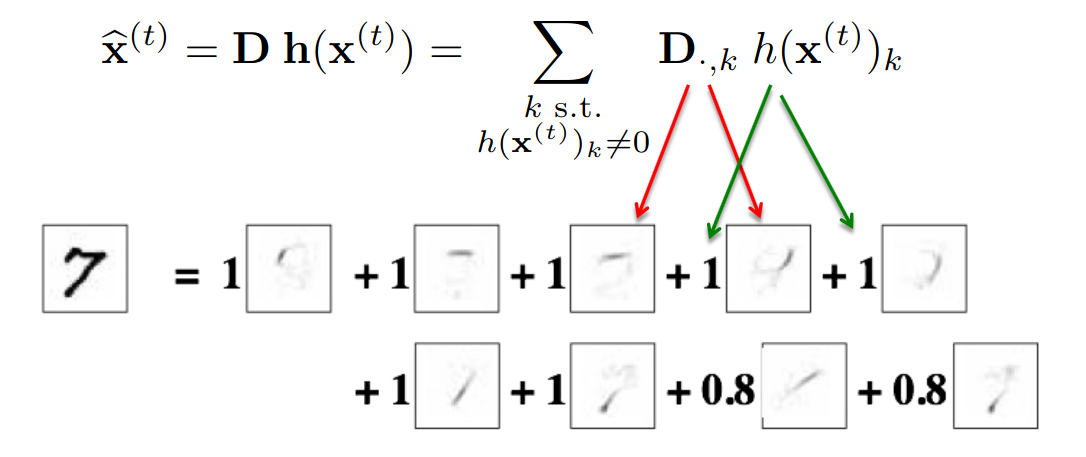
\includegraphics[scale=0.4]{img/sparse_coding.png}
    \caption{We can reconstruct an image of a seven as a linear combination of a set of images. Note that each of the images of strokes are columns of $W$ and the coefficients make up the sparse vector $h$. } 
    \label{fig:sparse_coding}
  \end{figure}

  Let's think about how we can optimize the objective function w.r.t. $h$, keeping $D$ constant. We can do stochastic gradient descent, which gives us the steps
  \begin{equation}
    \nabla_{h^{(t)}} \mathcal{L}(x^{(t)}) = D^T (D h^{(t)} - x^{(t)}) + \lambda \, \mathrm{sign}(h^{(t)})
  \end{equation}
  but this wouldn't achieve sparsity since it overshoots the $0$ all the time. Therefore, we can clip it, or we can use proximal gradient descent/ISTA to take a step, and shrink the parameters according to the L1 norm. 
  \begin{align} 
    h^{(t)} & = h^{(t)} - \alpha D^T (D h^{(t)} - x^{(t)}) \\
    h^{(t)} & = \mathrm{shrink}(h^{(t)}, \alpha \lambda)
  \end{align}
  where $\mathrm{shrink}(a, b) = [\ldots, \mathrm{sign}(a_i)\, \max(|a_i| - b_i, 0), \ldots]$. This is guaranteed to converge if $1/\alpha$ is bigger than the largest eigenvalue of $D^T D$.  

